
\chapter{Linguagens Livres do Contexto}\label{cap:LinguagemLLC}

\begin{introduction}[Tópicos]
	\item Gramática Livres do Contexto
	\item Simplificação e Formas Normais de GLC
	\item Sobre Algoritmos de Pertinência em GLC
	\item GLC e Linguagens de Programação
	\item Autômato de Pilha Determinístico
	\item Autômato de Pilha Não-determinístico
	\item Álgebra das Linguagens Livres de Contexto
	\item Questionário
\end{introduction}

No capítulo passado foram apresentadas três diferentes formalismos para a classe das linguagens regulares, a saber, o formalismo operacional (os autômatos), o formalismo denotacional (as expressões regulares) e por fim o formalismo gerador ou axiomático (as gramáticas regulares). Agora este manuscrito irá continuar o estudo das linguagens formais apresentando a classe das linguagens livres do contexto, como antes serão apresentados diferentes formalismo para tal classe de linguagens.

\section{Gramática Livres do Contexto}\label{sec:GLC}

O estudo das Linguagens Livres do Contexto será iniciado aqui pela apresentação de seu formalismo gerador, ou seja, será primeiro apresentado a noção de Gramática Livre do Contexto.

\begin{definition}[Gramática Livre do Contexto]\label{def:GLC}
	\cite{benjaLivro2010} Uma Gramática Livre do Contexto, ou simplesmente GLC, é uma gramática formal $G = \langle V, \Sigma, S, P\rangle$ onde todo $\alpha \rhd \beta \in P$ é tal que $\alpha \in V$ e $\beta \in (V \cup \Sigma)^*$.
\end{definition}

\begin{example}\label{exe:GLC-1}
	A estrutura $G = \langle \{A, B, C\}, \{0,1\}, A, P\rangle$ onde $P$ é definido pela regras:
	\begin{eqnarray*}
		A & \rhd & A0110BC \mid 0110C \mid AAB0110CC \mid \lambda\\
		B & \rhd & 01B10 \mid 0110\\
		C & \rhd & 01C \mid \lambda
	\end{eqnarray*}
	é uma GLC.
\end{example}

Obviamente o leitor atento pode notar que a Definição \ref{def:GLC} garante que toda Gramática Regular é um caso particular de GLC, porém o inverso não é verdadeiro, basta notar que a gramática apresentada no Exemplo \ref{exe:GLC-1}, fere a definição de gramática regular apresentada na Seção \ref{sec:GramaticaRegular} do capítulo passado. Agora utilizando a Definição \ref{def:LinaugemGramatica} pode-se formalizar o conceito de Linguagem Livre do Contexto.

\begin{definition}[Linguagem Livre do Contexto]\label{def:LLC}
	A linguagem $L$ gerada por uma GLC $G$, ou seja, $L = \mathcal{L}(G)$, será chamada de Linguagem Livre do Contexto, ou simplesmente LLC.
\end{definition}

Como para os casos das linguagens reconhecidas por AFD, para provar que uma determinada GLC $G$ gera uma linguagem $L$ é necessário demonstrar o seguinte resultado $w \in L \Longleftrightarrow w \in \mathcal{L}(G)$.

\begin{example}\label{exe:LinguagemGLC}
	A linguagem $L = \{a^ib^i \mid i  > 0\}$ é gerado pela GLC $G = \langle \{S\}, \{a,b,c\}, S, P\rangle$ onde $P$ é formado pelas regras,
	\begin{eqnarray*}
		S & \rhd & aSb \mid ab
	\end{eqnarray*}
	\begin{proof}
		$(\Rightarrow)$ Suponha que $w \in L$ assim $w = a^ib^i$ para $i  > 0$, agora por indução sobre a quantidade $n$ de derivações em $G$ será mostrado que toda forma sentencial gerada por $G$ é da forma $a^nS^jb^n$ com $j \in \{0, 1\}$. 
		\begin{itemize}
			\item[ ] \textbf{Base da indução}: Com $n = 1$, é trivial pelas regras em $P$. 
			\item[ ] \textbf{Hipótese indutiva (HI)}: Assuma que com $n$ derivações tal que $n \geq 0$ a forma sentencial $a^nS^jb^n$ é gerada pela GLC $G$, ou seja, $S \gg^n a^nS^jb^n$ com $j \in \{0, 1\}$. 
			\item[ ] \textbf{Passo indutivo}: Agora dado $S \gg^{n+1} w'$, ou seja, $w'$ é derivada de $S$ com $n+1$ derivações, assim por definição tem-se que existe $w''$ tal que $S \gg^n w'' \gg w'$, mas por \textbf{(HI)} tem-se que $w'' =  a^nS^jb^n$ com $n \geq 0$ e $j \in \{0, 1\}$,  desde que, $w'$ é gerada de $w''$ é claro que $j = 1$, ou seja, $w'' = a^nSb^n$, consequentemente, $w' = a^{n+1}Sb^{n+1}$ ou $w' = a^{n+1}b^{n+1}$ e, portanto, $w'$ é da forma $a^{n+1}S^jb^{n+1}$ com $j \in \{0, 1\}$. 
		\end{itemize}
		Agora por hipótese tinha-se que $w = a^ib^i$ para $i  > 0$, ou seja, $w = a^iS^0b^i$, dessa forma pela indução acima $w$ é uma forma sentencial gerada por $G$, e como $w \in \Sigma^*$ tem-se por definição que $w \in \mathcal{L}(G)$. $(\Rightarrow)$ Suponha que $w \in \mathcal{L}(G)$, agora será mostrado por indução sobre a quantidade $n$ de derivações que todo $w$ gerado por $G$ estará em $L$.
		\begin{itemize}
			\item[ ] \textbf{Base da indução:} Com $n=1$, ou seja, como uma única derivação, pelo fato de que $w \in \Sigma^*$ e pelas regras em $P$ tem-se obrigatoriamente que $w = ab$ e, portanto, $w = a^1b^1$ , consequentemente, $w \in L$.
			\item[ ] \textbf{Hipótese indutiva (HI)}: Assuma que para todo $S \gg^n w$ tal que $n \geq 1$, tem-se que $w \in L$.
			\item[ ] \textbf{Passo indutivo}: Agora dado $S \gg^{n+1} w$, ou seja, $w$ é derivado em $G$ com $n + 1$ derivações de forma que $n \geq 1$. Desde que $n  \geq 1$ tem-se que $n + 1  > 1$, assim a palavra $ab$ não pode ser $w$ uma vez que são usadas pelo menos duas derivações para gerar $w$. Assim a derivação de $w$ deverá ter sido iniciado usando a regra $S \rhd aSb$ e, portanto, $w = aw'b$ em que $S \gg^n w'$, mas pela hipótese indutiva $w' \in L$, logo $w' = a^ib^i$ com $i > 0$, consequentemente $w = aa^ib^ib = a^{i+1}b^{i+1}$, logo $w \in L$.
		\end{itemize}
	\end{proof}
\end{example}

Note que para a prova mostrada no Exemplo \ref{exe:LinguagemGLC} foi-se usada indução sobre o tamanho das derivações, isto não é a única forma de se proceder para provar que uma gramática gera uma determinada linguagem, de  fato como apresentado em \cite{hopcroft2008} pode-se usar a ideia de indução sobre as árvores de derivações (apresentadas mais a frente), neste manuscrito não será apresentado tal estratégia, porém fica a referência para interessados no tema. 

Nas GLC que não são lineares, ou seja, as gramática em que as regras em $P$ podem conter duas ou mais variáveis do lado direto do símbolo $\rhd$, é permitido a escolha sobre qual variável ser derivada primeiramente, para ilustrar isso considere uma forma sentencial $0A10BC$ e as regras $A \rhd 00, B \rhd \lambda$ e $C \rhd 1$, note que dependendo de qual variável é escolhida para ser reescrita a próxima forma sentencial pode assumir três formas diferentes. Apresentado esta ideia pode-se agora formalizar o conceito de reescrita \textbf{mais à esquerda} e \textbf{mais à direita}.

\begin{definition}[Tipos de Derivação]\label{def:TiposLateraisReescrita}
	Dado uma GLC $G = \langle V, \Sigma, S, P\rangle$ e seja $w_1A_1w_2\cdots w_nA_nw_{n+1}$ uma forma sentencial derivável em $G$ tal que $w_i \in \Sigma^*$ e $A_j \in V$ para todo $1 \leq i \leq n+1$ e $1 \leq j \leq n$. Uma derivação é dita mais à esquerda (à direita) se ela é da forma $w_1A_1w_2\cdots w_nA_nw_{n+1} \gg w_1w'w_2\cdots w_nA_nw_{n+1}$ ($w_1A_1w_2\cdots w_nA_nw_{n+1} \gg w_1A_1w_2\cdots w_nw'w_{n+1}$)  com  $w' \in (V \cup \Sigma)^*$.
\end{definition}

\begin{example}\label{exe:ReescritasLaterais}
	Considere a GLC $G = \langle \{S, A, B\}, \{0, 1\}, S, P\rangle$ em que $P$ é formado pelas regras,
	\begin{eqnarray*}
		S & \rhd & 0AB\\
		A & \rhd & 11B1 \\
		B & \rhd & A \mid \lambda 
	\end{eqnarray*}
	claramente a palavra $011B1A$ é um forma sentencial derivável em $G$, agora note que:
	\begin{eqnarray*}
		011B1A & \gg & 011A1A\\
		011B1A & \gg & 0111A
	\end{eqnarray*}
	são ambas derivações mais à esquerda, e 
	\begin{eqnarray*}
		011B1A & \gg & 011B111B1
	\end{eqnarray*}
	é uma derivação mais à direita.
\end{example}

\begin{definition}[Tipo de Geração]\label{def:TipoGeracao}
	Dado uma GLC $G = \langle V, \Sigma, S, P\rangle$,  uma derivação $S \gg^* w$ é dita ser uma geração mais à esquerda (à direita) sempre que $w \in \Sigma^*$ e toda derivação realizada for mais à esquerda (à direita).
\end{definition}

\begin{example}\label{exe:TipoGeracao}
	Considere a gramática do Exemplo \ref{exe:ReescritasLaterais} a derivação, 
	$$S \gg 0AB \gg 011B1B \gg 0111B \gg 0111$$
	é claramente uma geração mais à esquerda, já a derivação
	$$S \gg 0AB \gg 0A \gg 011B1 \gg 0111$$
	é notavelmente uma geração mais à direita.
\end{example}

\begin{remark}
  Resumindo dado uma GLC $G = \langle V, \Sigma, S, P\rangle$ uma geração é obrigatoriamente uma derivação $S \gg w$ em que $w \in \Sigma^*$, ou seja, uma derivação que gera (ou produz) uma palavra sobre o alfabeto $\Sigma$.
\end{remark}

Além da noção de geração, para visualizar o passo a passo da ``construção'' de uma palavra $w \in \Sigma^*$ em uma GLC $G$ é comum usar a ideia de árvore de derivação\footnote{Na literatura como no livro \cite{benjaLivro2010} também é comum encontrar a nomenclatura árvore ordenada.}. 

Uma árvore de derivação nada mais é do que uma forma visual estruturada em uma árvore\footnote{As árvores de derivação são representações cuja a forma similar a construção das árvores $n$-árias da área de estrutura de dados \cite{jaime1994}.} que representar a construção de uma palavra, em que cada nível da árvore representa é gerada pela aplicação de uma ou mais regras de reescrita, neste sentido as folhos da árvore contém os símbolos da palavra $w$.

\begin{definition}[Árvore de Derivação]\label{def:ArvoreGLC}
	Seja $G = \langle V, \Sigma, S, P\rangle$ uma GLC e dado $w \in \mathcal{L}(G)$, uma árvore de derivação para $w$ é construída seguindo as seguintes regras:
	\begin{enumerate}
		\item O símbolo $S$ é a raiz da árvore.
		\item Todo símbolo $a \in \Sigma \cup \{\lambda\}$ é o rótulo de uma folha.
		\item Todo símbolo $A \in V$ é o rótulo de uma raiz de uma sub-árvore\footnote{Aqui sub-árvore e no mesmo sentido que o leitor já deve ter visto em estrutura de dados.}.
		\item Se $A$ é uma raiz e seus ``filhos'' são  $x_1, \cdots, x_n$ com $x_i \in V \cup \Sigma \cup \{\lambda\}$ para $1 \leq i \leq n$, então existe em $P$ uma regra da forma $A \rhd x_1\cdots x_n$.
		\item Todo folha rotulada por $\lambda$ de uma raiz $A$ será filho único, ou seja, em $P$ existe uma regra da forma $A \rhd \lambda$.
	\end{enumerate}
\end{definition}

\newpage
\begin{example}\label{exe:ArvoreGLC1}
	Tem-se que a derivação $S \gg 0AB \gg 011B1B \gg 0111B \gg 0111$ apresentada no Exemplo \ref{exe:TipoGeracao} é representada pela árvore esboçada na Figura \ref{fig:ArvoreGLC1} a seguir.
	
	\begin{figure}[h]
		\centering
		\begin{tikzpicture}[sibling distance=.6cm, empty/.style={draw=none}, tlabel/.style={font=\footnotesize\color{red!70!black}}]
			\Tree   [.$S$  
					[.$0$ ]
						%\edge node[tlabel,auto=left] {1}; 
					[.$A$  
							[.$1$ ]
							[.$1$ ]
							[.$B$ 
								{$\lambda$}
							] 
							[.$1$ ]
					] 
					[.B   
						%\edge[empty]; {} \edge node[tlabel,auto=left] {5}; {b}   
						{$\lambda$}
					]
			]
		\end{tikzpicture}
		\caption{Árvore para a derivação $S \gg 0AB \gg 011B1B \gg 0111B \gg 0111$.}
		\label{fig:ArvoreGLC1}
	\end{figure}
\end{example}

\begin{example}\label{exe:ArvoreGLC2}
	Tem-se que a derivação $S \gg 0AB \gg 0A \gg 011B1 \gg 0111$ apresentada no Exemplo \ref{exe:TipoGeracao} é representada pela árvore esboçada na Figura \ref{fig:ArvoreGLC2} a seguir.
	
	\begin{figure}[h]
		\centering
		\begin{tikzpicture}[sibling distance=.6cm, empty/.style={draw=none}, tlabel/.style={font=\footnotesize\color{red!70!black}}]
			\Tree [.$S$  
					[.$0$ ]
					[.$A$
						[.$1$ ] 
						[.$1$ ] 
						[.$B$ 
							{$\lambda$}
						] 
						[.$1$ ] 
					]
					[.$B$
						{$\lambda$} 
					]
			]
		\end{tikzpicture}
		\caption{Árvore para a derivação $S \gg 0AB \gg 0A \gg 011B1 \gg 0111$.}
		\label{fig:ArvoreGLC2}
	\end{figure}
\end{example}

\begin{remark}
	Os Exemplos \ref{exe:ArvoreGLC1} e \ref{exe:ArvoreGLC2} mostram que que diferentes derivações podem ser representadas pela mesma árvore, isso acontece devido ao fato de que a árvore de derivação apenas esboça o processo de formação total (ou final), e não o comportamento (ou momento) parcial das derivação.
\end{remark}

\begin{note}
	Em algumas obras tais como \cite{benjaLivro2010} as folhas e raízes nas árvores de derivação são gravados com círculos, neste manuscrito isso não será feito para não confundir o leitor iniciante com a representação visual dos autômatos finitos.
\end{note}

\begin{definition}[Ambiguidade]\label{def:AmbiguidadePalavra}
	Dado uma GLC $G = \langle V, \Sigma, S, P\rangle$ uma palavra $w \in \mathcal{L}(G)$ é dita ser ambígua sempre que existe duas gerações diferentes para $w$.
\end{definition}

A Definição \ref{def:AmbiguidadePalavra} pode ser reinterpretada da seguinte forma: uma palavra $w$ é ambígua com relação a uma GLC $G$ se existem duas gerações mais à esquerda (à direta) para tal palavra.

\begin{definition}[Linguagem Ambígua]\label{def:LinguagemAmbiguidade}
	Uma linguagem $L$ é dita ser ambígua se existe uma GLC $G$ e uma palavra $w$ tal que $L = \mathcal{L}(G)$ e $w$ seja uma palavra ambígua em $G$. L será dita inerentemente ambígua se existe $w$ para todo GLC $G$ tal que  $w$ seja uma palavra ambígua em $G$ e $L = \mathcal{L}(G)$.
\end{definition}

\begin{example}
	Considere a GLC $G = \langle \{S\}, \{a, b\}, S, P \rangle$ onde $P$ é o formado pelas seguintes regras:
	\begin{eqnarray*}
		S & \rhd & aSb \mid SS \mid \lambda
	\end{eqnarray*}
	a palavra $aabb$ é ambígua, pois existem as duas árvores de derivação apresentadas na Figura \ref{fig:ArvoresAmbuigas}, assim tem-se que $\mathcal{L}(G)$ é uma linguagem ambígua.
	
	\begin{figure}[h]
		\centering
		\subfloat[Primeira ávore.]{
			\begin{tikzpicture}[sibling distance=.8cm, empty/.style={draw=none}, tlabel/.style={font=\footnotesize\color{red!70!black}}]
				\Tree [.$S$  
						[.$a$ ]
						[.$S$
							[.$a$ ] 
							[.$S$
								{$\lambda$} 
							] 
							[.$b$ ] 
						]
						[.$b$ ]
				]
			\end{tikzpicture}
			\label{Ima:Arvore1}
		}\hfill
		\subfloat[Segunda ávore.]{
			\begin{tikzpicture}[sibling distance=.8cm, empty/.style={draw=none}, tlabel/.style={font=\footnotesize\color{red!70!black}}]
				\Tree [.$S$  
						[.$S$
							{$\lambda$} 
						]
						[.$S$
							[.$a$ ]
							[.$S$
								[.$a$ ] 
								[.$S$
									{$\lambda$} 
								] 
								[.$b$ ] 
							]
							[.$b$ ] 
						]
				]
			\end{tikzpicture}
			\label{Ima:Arvore2}
		}%
		\caption{As árvores de derivação para a palavra $aabb$}
		\label{fig:ArvoresAmbuigas}
	\end{figure}
\end{example}

Ambiguidade é uma característica comum encontrada nas linguagem naturais \cite{benjaLivro2010} e em tais linguagens essa característica é tolerada, em contrapartida, as linguagens de programação não toleram muito bem o aspecto da ambiguidade assim em geral a mesma deve ser sempre que possível evitada ou eliminada. Uma estratégia comum para a eliminação da ambiguidade em linguagens de programação é estabelecer prioridade na geração de certos símbolos da linguagens \cite{benjaLivro2010, aho2007}. 

\section{Simplificação de Gramática Livres do Contexto}\label{sec:SimplficacaoGLC}

Antes de apresentar as regras de simplificação e alguns resultados sobre as mesmas é conveniente discutir alguns aspectos sobre as GLC. Antes de tudo lembre que na definição de GLC (Definição \ref{def:GLC}) não existe qualquer restrição para a forma das palavras encontradas à direita das regras de reescrita. Assim podem haver $n$ variáveis, recursão, geração de $\lambda$ e etc. Algumas desta, entretanto, podem ser removidas ou alteradas de forma que a gramática possa ser mais simples de ser utilizada, e será isto que será estudado nesta seção, ou seja, aqui será estudado diversas estratégias para transformar uma gramática qualquer $G$ em uma gramática $G'$ com alguns restrições, mas que preserva a linguagem gerada, isto é, $\mathcal{L}(G) = \mathcal{L}(G')$. 

\begin{remark}
    Assim como em \cite{benjaLivro2010} as gramáticas que serão consideradas nesta seção não são capazes de gerar a palavra vazia, ou seja, $S \not\gg \lambda$ ou ainda $\lambda \notin \mathcal{L}(G)$. Entretanto isso não irá diminuir em nada a força dos resultados que serão obtidos aqui.
\end{remark}

\begin{definition}[Regra da substituição]\label{def:RegraSubstituicao}
    Seja $G = \langle V, \Sigma, S, P\rangle$ uma GLC e seja $A, B \in V$ tal que $A \neq B$ de forma que em $P$ existem as produções:
    $$A \rhd x_1Bx_2$$
    e
    $$B \rhd y_1 \mid y_2 \mid \cdots \mid y_n$$
    a regra de substituição consiste em para cada a regra $A \rhd x_1A x_2$ em $P$ adicionar as regras:
    $$A \rhd x_1y_1x_2 \mid x_1y_2x_2 \mid \cdots \mid x_1y_nx_2 \mid$$.
\end{definition}

Note que a regra de substituição de fato só altera a forma do conjunto $P$ gerando um novo conjunto $P'$, e pela própria regra é fácil notar que vale a seguinte desigualdade $\# P \leq \# P'$. 

\begin{theorem}\label{teo:SuplificacaoGLC-Sub}
    Se $G = \langle V, \Sigma, S, P\rangle$ é uma GLC, então a gramática $G'$ gerada a partir da regra de substituição é tal que $\mathcal{L}(G) = \mathcal{L}(G')$.
\end{theorem}

\begin{proof}
    Suponha $G = \langle V, \Sigma, S, P\rangle$ é uma GLC, agora seja $G' = \langle V, \Sigma, S, P'\rangle$ a GLC gerada a partir da regra de substituição aplicada a $G$. Agora assuma que $w \in \mathcal{L}(G)$, ou seja, $S \gg_G^* w$, dessa forma há dois casos para serem considerados:
    \begin{itemize}
        \item[(1)] Se durante a derivação $S \gg_G^* w$ não forem usadas regras da forma $A \rhd x_1Bx_2$, então obviamente essa mesma derivação pode ser replicada em todos os seu detalhes na gramática $G'$, uma vez que, todas as regras que não são da forma $A \rhd x_1Bx_2$ estão também em $P'$, assim $S \gg_{G'}^* w$, consequentemente, $w \in \mathcal{L}(G')$.
        \item[(2)] Agora sem perda de generalidade assuma que pelo menos uma regra da forma  $A \rhd x_1Bx_2$ seguida da regra $B \rhd y_1$ aparecem na derivação $S \gg_G^* w$, portanto, tem-se que:
        $$S \gg_G^* k_1Ak_2 \gg_{G} k_1x_1Bx_2k_2 \gg_{G} k_1x_1y_1x_2k_2 \gg^*_G w $$
        com $k_1, k_2, x_1, x_2, y_1 \in (V \cup \Sigma)^*$. Assim pela construção de $G'$ pode-se então realizar a seguinte derivação:
        $$S \gg^*_{G'} k_1Ak_2 \gg_{G'} k_1x_1y_1x_2k_2  \gg^*_{G'} w$$
        e assim tem-se que, $w \in \mathcal{L}(G')$.
    \end{itemize}
    Logo pelos casos $(1)$ e $(2)$ acima tem-se que $\mathcal{L}(G) \subseteq \mathcal{L}(G')$. Agora mostrar que $\mathcal{L}(G') \subseteq \mathcal{L}(G)$ é trivial e não será feito aqui, e desde que $\mathcal{L}(G) \subseteq \mathcal{L}(G')$ e $\mathcal{L}(G') \subseteq \mathcal{L}(G)$ por definição tem-se que $\mathcal{L}(G) = \mathcal{L}(G')$ o que completa a prova.
\end{proof}

Como pode ser visto no Teorema \ref{teo:SuplificacaoGLC-Sub} e como discutido em \cite{benjaLivro2010} a regra de substituição pode até aumentar o número de regras de reescrita, porém, a mesma também permite que seja realizadas geração mais rápidas, isto é, que aconteçam derivações de palavras $w \in \Sigma^*$ com menos passos.

\begin{example}
    Dado a GLC $G = \langle \{S, A, B, C\}, \{0,1\}, S, P \rangle$ com $P$ definido pelas regras:
    \begin{eqnarray*}
        S & \rhd & A001 \mid B100\\
        A & \rhd & 01 \mid 01B\\
        B & \rhd & 1 \mid 0 \mid \lambda
    \end{eqnarray*}
    aplicando a regra de substituição em tal gramática será gerada na gramática $G' = \langle \{S, A, B, C\}, \{0,1\}, S, P' \rangle$ em que $P'$ corresponde ao conjunto formado pela seguintes regras:
    \begin{eqnarray*}
        S & \rhd & A001 \mid B100 \mid  01001 \mid 01B001 \mid 1100 \mid 0100 \mid 100 011001 \mid 010001 \mid 01001\\
        A & \rhd & 01 \mid 01B \mid 011 \mid  010 \\
        B & \rhd & 1 \mid 0 \mid \lambda
    \end{eqnarray*}
\end{example}

Para prosseguir com o estudo das regras de simplificação antes é necessário formalizar o conceito de variável recursiva à esquerda nas GLC.

\begin{definition}[Regra Recursiva à Esquerda]\label{def:VariavelRecursiva}
    Seja $G = \langle V, \Sigma, S, P\rangle$ uma GLC, uma variável $A$ é dita recursiva à esquerda se existe pelo menos uma regra $A \rhd Ax \in P$ com  $A \in V$ e $x \in (V \cup \Sigma)^*$.
\end{definition}

Agora é possível formalizar então a próxima regra de simplificação de GLC, sendo esta próxima regra nomeada como \textbf{Regra de Remoção da Recursividade Esquerda}.

\begin{definition}[Regra de Remoção da Recursividade Esquerda]\label{def:RegraRecursiva}
    Seja $G = \langle V, \Sigma, S, P\rangle$ uma GLC com variáveis recursivas à esquerda. Então substitua para cada $A \in V$ as regras:
    $$A \rhd Ax_1 \mid \cdots \mid Ax_m \mid y_1 \mid \cdots \mid y_n$$
    pelas regras:
    \begin{eqnarray*}
        A & \rhd & y_1 \mid \cdots \mid y_n \mid y_1Z \mid \cdots \mid y_nZ\\
        Z & \rhd & x_1 \mid \cdots \mid x_m \mid x_1Z \mid \cdots \mid x_mZ
    \end{eqnarray*}
	onde $x_1, \cdots, x_m, y_1, \cdots, y_n \in (V \cup \Sigma)^*$ e $Z$ é uma variável nova que deve ser adicionada ao conjunto $V$.
\end{definition}

Fica claro pela definição da Regra de Remoção da Recursividade Esquerda que após usa aplicação será gerada uma nova gramática com mais varáveis que a gramática original terá uma quantidade igual ou superior de regras de reescritas.

\begin{theorem}\label{teo:SuplificacaoGLC-Rec}
    Se $G = \langle V, \Sigma, S, P\rangle$ é uma GLC, então a gramática $G'$ gerada a partir da regra de remoção da recursividade esquerda é tal que $\mathcal{L}(G) = \mathcal{L}(G')$.
\end{theorem}

\begin{proof}
    Ficará como exercício ao leitor.
\end{proof}

\begin{example}
    Dado a GLC $G = \langle \{S, A\}, \{a,b, c\}, S, P \rangle$ com $P$ definido pelas regras:
    \begin{eqnarray*}
        S & \rhd & aSc \mid aAc\\
        A & \rhd & Ab \mid b
    \end{eqnarray*}
    Usando a regra de remoção da recursividade esquerda é obtida a GLC $G = \langle \{S, A, B\}, \{a, b, c\}, S, P' \rangle$ onde $P'$ é definido por:
    \begin{eqnarray*}
        S & \rhd & aSc \mid aAc\\
        A & \rhd & b \mid bB\\
        B & \rhd & b \mid bB 
    \end{eqnarray*}
\end{example}

Agora para continuar com o estudo das regras de simplificação será necessário formalizar três conceitos chaves, o primeiro conceito é a noção de relação (ou grafo) de dependências, a saber tais relações (ou grafos) são ferramentas advindas da teoria dos grafos e frequentemente usada em muitos campos do conhecimento para modela sistemas complexos \cite{benjaLivro2010}, a seguir este conceito será apresentado de forma rigorosa com respeito as GLC.

\begin{definition}[Relação de dependência]\label{def:GrafoDependencia}
    Seja $G = \langle V, \Sigma, S, P\rangle$ é uma GLC, a relação de dependência $DEP$ é construída como: $(A, B) \in DEP$ se, e somente se, $A \rhd xBy \in P$ com $x, y \in (V \cup \Sigma)^*$ e $A \neq B$.
\end{definition}

O leitor pode considerar a relação $DEP$ como sendo uma relação de necessidade, em que $(A, B) \in DEP$ pode ser semanticamente interpretado como, para escrever $B$ é necessário que antes existem um $A$.

\begin{remark}
    Para fins de notação, será usado o rótulo $\widehat{DEP}$ para denotar o fecho transitivo da relação $DEP$.
\end{remark}

\begin{example}\label{exe:GLCDEP}
    Considere a GLC $G = \langle \{A, B, C, D, E\}, \{0, 1\}, A, P \rangle$ onde $P$ é o conjunto formado pelas regras:
    
    \begin{eqnarray*}
        A & \rhd & 00A \mid 0B1 \mid 10AB \mid AD\\ 
        B & \rhd & 1B01 \mid D01E\mid \lambda\\
        C & \rhd & C01 \mid 00101 \mid 1 \mid \lambda\\
        D & \rhd & 01E \mid 0E\\
        E & \rhd & 1E0 \mid EE \mid D
    \end{eqnarray*}
    Tem-se que $\widehat{DEP}$ é o conjunto formado pelo pares $(A, B), (A, D), (B, D), (B, E), (D, E),$ e $(E, D)$.
\end{example}

O próximo conceito necessário é a noção de variável inacessível formalizado a seguir.

\begin{definition}[Variável inacessível]\label{def:VariavelInacessível}
    Seja $G = \langle V, \Sigma, S, P\rangle$ é uma GLC, uma variável $A \neq S$ é dita ser inacessível sempre que $(S, A) \notin \widehat{DEP}$.
\end{definition}

\begin{example}
    Considere a GLC apresentada no Exemplo \ref{exe:GLCDEP}, em tal gramática é fácil notar que a variável $C$ é inacessível.
\end{example}

\begin{lemma}\label{lema:SemInacessivel}
    Se $G = \langle V, \Sigma, S, P\rangle$ é uma GLC, então existe uma GLC sem variáveis inacessíveis $G' = \langle V', \Sigma, S, P'\rangle$ tal que $\mathcal{L}(G) = \mathcal{L}(G')$.
\end{lemma}

\begin{proof}
    Suponha que $G = \langle V, \Sigma, S, P\rangle$ é uma GLC, assim pode-se construir uma nova GLC $G' = \langle V', \Sigma, S, P'\rangle$ onde: 
    \begin{itemize}
        \item $V' = V - \{A \in V \mid A \mbox{ é uma variável inacessível}\}$ e
        \item $P' = \{A \rhd xBy \in P \mid A, B \in V', x, y \in (V' \cup \Sigma)^*\}$.
    \end{itemize}
    Agora é claro que $G'$ possui apenas variáveis acessíveis. Note agora que para toda $S \gg_G w$ tem-se que apenas regras com variáveis acessíveis são utilizadas em tal derivação, além disso, é claro pela construção de $G'$ que tais regras estarão em $P'$, consequentemente $S \gg_{G'} w$, assim $\mathcal{L}(G) \subseteq \mathcal{L}(G')$. Por outro lado, assuma por absurdo que $\mathcal{L}(G') \not\subseteq \mathcal{L}(G)$, assim existe um $w \in \mathcal{L}(G')$ tal que $w \notin \mathcal{L}(G)$, desde que $w \in \mathcal{L}(G')$ tem-se que $S \gg_{G'} w$, mas pela construção de $G'$ é obvio que toda regra usada na derivação $S \gg_{G'} w$ também estão presente em $P$ e, portanto, $S \gg_{G} w$ o que contradiz a hipótese de que $\mathcal{L}(G') \not\subseteq \mathcal{L}(G)$, consequentemente, tem-se $\mathcal{L}(G') \subseteq \mathcal{L}(G)$. Desde que, $\mathcal{L}(G) \subseteq \mathcal{L}(G')$ e $\mathcal{L}(G') \subseteq \mathcal{L}(G)$, pela definição de igualdade entre conjunto tem-se que $\mathcal{L}(G) = \mathcal{L}(G')$.
\end{proof}

O terceiro e último conceito necessário para continuar com o estudo das regras de simplificação é a ideia de variável descartável em uma GLC, de forma direta uma variável descartável é aquela incapaz de derivar uma palavra sobre o alfabeto $\Sigma$, em notação formal tem-se a definição a seguir.

\begin{definition}[Variável descartável]\label{def:VariavelDescartavel}
    Seja $G = \langle V, \Sigma, S, P\rangle$ é uma GLC, uma variável $A$ é dita descartável sempre que para todo $w \in \Sigma^*$ tem-se que $A \not\gg^* w$.
\end{definition}

\begin{example}
    Considere a GLC apresentada no Exemplo \ref{exe:GLCDEP}, em tal gramática as variáveis $D$ e $E$ são ambas descartáveis.
\end{example}

O leitor um pouco mais experiente em programação pode facilmente notar que uma variável descartável é aquela que é a raiz de uma árvore infinita, isto é, uma árvore que continua crescendo infinitamente, outra forma de interpretar uma variável descartável é como sendo uma variável que produz um \textit{loop} infinito no processo de derivação, ou seja, a partir de tal variável nunca é possível derivar uma palavra sobre o alfabeto base da gramática.

\begin{lemma}\label{lema:SemDescartavel}
    Se $G = \langle V, \Sigma, S, P\rangle$ é uma GLC, então existe uma GLC sem variáveis descartável $G' = \langle V', \Sigma, S, P'\rangle$ tal que $\mathcal{L}(G) = \mathcal{L}(G')$.
\end{lemma}

\begin{proof}
    Suponha que $G = \langle V, \Sigma, S, P\rangle$ é uma GLC, assim pode-se construir uma nova GLC $G' = \langle V', \Sigma, S, P'\rangle$ onde: 
    \begin{itemize}
        \item $V' = V - \{A \in V \mid A \mbox{ é uma variável descartável}\}$ e
        \item $P' = \{A \rhd xBy \in P \mid A, B \in V', x, y \in (V' \cup \Sigma)^*\}$.
    \end{itemize}
    Agora é claro que $G'$ não possui variáveis descartáveis. A argumentação para provar $\mathcal{L}(G) = \mathcal{L}(G')$ é similar a demonstração do Lema \ref{lema:SemInacessivel}.
\end{proof}

\begin{definition}[Regra de remoção de variáveis inúteis]\label{def:RegraInuteis}
    Dado uma GLC $G = \langle V, \Sigma, S, P\rangle$ será gerada uma gramática $G'$ sem variáveis inúteis, após a execução dos seguintes passos.
    \begin{enumerate}
        \item Remova todas as variáveis Descartáveis e assim gere uma gramática $G_1$.
        \item Remova da gramática $G_1$ todas as variáveis Inacessíveis, e assim gere a gramática $G'$.
    \end{enumerate}
\end{definition}

O termo inútil diz respeito ao fato de uma variável $A$ não ser capaz de derivar uma palavra $w \in \Sigma^*$, ou seja, $A \not\gg_G w$.

\begin{theorem}\label{teo:SemVariaveisInuteis}
    Se $G = \langle V, \Sigma, S, P\rangle$ é uma GLC, então a GLC $G'$ gerada pela regra de remoção de variáveis inúteis é tal que $\mathcal{L}(G) = \mathcal{L}(G')$.
\end{theorem}

\begin{proof}
    Direto dos Lemas \ref{lema:SemInacessivel} e \ref{lema:SemDescartavel}.
\end{proof}

O exemplo a seguir ilustra a aplicação da regra de remoção de variáveis inúteis.

\begin{example}
    Considere a GLC $G = \langle \{S, T, V, X, Y, Z\}, \{0, 1\}, S, P \rangle$ onde $P$ é o conjunto com as seguintes produções:
    \begin{eqnarray*}
        S & \rhd & 01S \mid SX0 \mid YZ \mid X0Z11\\
        T & \rhd & \lambda\\
        X & \rhd & X01 \mid Y0X\\
        Y & \rhd & S01 \mid YY \mid XY \mid \lambda\\
        Z & \rhd & S01 \mid SS
    \end{eqnarray*}
    Removendo as variáveis descartáveis (neste caso existe apenas variável $X$ a ser removida)  é gerado a GLC $G_1 = \langle \{S, T, V, Y, Z\}, \{0, 1\}, S, P_1 \rangle$ com $P_1$ sendo:
    \begin{eqnarray*}
        S & \rhd & 01S \mid YZ \\
        T & \rhd & \lambda\\
        Y & \rhd & S01 \mid YY \mid \lambda\\
        Z & \rhd & S01 \mid SS
    \end{eqnarray*}
    Agora trabalhando considerando o conjunto $P_1$ pode-se remover as variáveis inacessíveis, ou seja, são removidas as variáveis $T, V$ e assim tem-se como resultado final da remoção de variáveis inúteis é gerada a GLC $G' = \langle \{S, Y, Z\}, \{0, 1\}, S, P' \rangle$ onde $P'$ é formado por:
    \begin{eqnarray*}
        S & \rhd & 01S \mid YZ \\
        Y & \rhd & S01 \mid YY \mid \lambda\\
        Z & \rhd & S01 \mid SS
    \end{eqnarray*}
\end{example}

\begin{definition}
    Seja $G = \langle V, \Sigma, S, P\rangle$ é uma GLC, uma regra da forma $A \rhd \lambda$ é chamada de $\lambda$-produção. 
\end{definition}

O próximo resultado estabelece que em GLC a existência de $\lambda$-produções não aumenta o poder gerativo das gramáticas.

\begin{theorem}\label{teo:SemLambdaProducoes}
    Se $G = \langle V, \Sigma, S, P\rangle$ é uma GLC, então existe uma GLC $G'$ sem $\lambda$-produções tal que $\mathcal{L}(G) = \mathcal{L}(G')$.
\end{theorem}

\begin{proof}
    Suponha que $G = \langle V, \Sigma, S, P\rangle$ é uma GLC, agora defina os conjuntos 
    \begin{eqnarray*}
        P_1  & = &  P - \{A \rhd \lambda \mid A \in V\}\\
        V_\lambda & = &  \{A \in V \mid A \rhd \lambda\}
    \end{eqnarray*}
    Pode-se agora construir um novo conjunto de regras $P_2$ da seguinte forma,  para cada uma das regras
    $$A \rhd w_1A_1w_2A_2w_3\cdots w_{n-1}A_{n-1}w_{n}A_nw_{n+1} \in P_1$$
    com $w_i \in (V \cup \Sigma)^*, A_j \in V_\lambda$ sendo $1 \leq i \leq n+1$ e $1 \leq j \leq n$ estarão em $P_2$ as regras:
    \begin{eqnarray*}
        A & \rhd & w_1w_2A_2w_3\cdots w_{n-1}A_{n-1}w_{n}A_nw_{n+1}\\
        A & \rhd & w_1A_1w_2w_3\cdots w_{n-1}A_{n-1}w_{n}A_nw_{n+1}\\
        \vdots & \vdots & \hspace{2.7cm} \vdots\\
        A & \rhd & w_1A_1w_2A_2w_3\cdots w_{n-1}w_{n}A_nw_{n+1}\\
        A & \rhd & w_1A_1w_2A_2w_3\cdots w_{n-1}A_{n-1}w_{n}w_{n+1}\\
        A & \rhd & w_1w_2w_3\cdots w_{n-1}w_{n}w_{n+1} 
    \end{eqnarray*}
    Finalmente defina a GLC $G' = \langle V, \Sigma, S, P' \rangle$ em que $P' = P_1 \cup P_2$, é claro por sua construção que $P'$ não possui $\lambda$-produções. Agora assuma que $w \in \mathcal{L}(G)$, ou seja, $S \gg_G^* w$, dessa forma há dois casos para serem considerados:
    \begin{itemize}
        \item[(1)] Se durante a derivação $S \gg_G^* w$ não forem usadas regras da forma $A \rhd \lambda$, então obviamente essa mesma derivação pode ser replicada em todos os seu detalhes na gramática $G'$, uma vez que, todas as regras que não são da forma $A \rhd \lambda$ estão também em $P'$, assim $S \gg_{G'}^* w$, consequentemente, $w \in \mathcal{L}(G')$.
        \item[(2)] Agora sem perda de generalidade assuma que pelo menos uma regra da forma  $A \rhd x_1Bx_2$ seguida da regra $B \rhd \lambda$ aparecem na derivação $S \gg_G^* w$, portanto, tem-se que:
        $$S \gg_G^* k_1Ak_2 \gg_{G} k_1x_1Bx_2k_2 \gg_{G} k_1x_1x_2k_2 \gg^*_G w $$
        com $k_1, k_2, x_1, x_2,  \in (V \cup \Sigma)^*$. Assim pela construção de $G'$ existe uma regra da forma $A \rhd x_1x_2$ e, portanto, em $G'$ é possível realizar a seguinte derivação
        $$S \gg_G^* k_1Ak_2 \gg_{G'} k_1x_1x_2k_2 \gg^*_G w $$
        e assim tem-se que $w \in \mathcal{L}(G')$.
    \end{itemize}
    Assim pelos casos $(1)$ e $(2)$ mostrados acima tem-se que $\mathcal{L}(G) \subseteq \mathcal{L}(G')$. Por outro lado, mostrar que $\mathcal{L}(G') \subseteq \mathcal{L}(G)$ é trivial e ficará como exercício ao leitor. Desde que $\mathcal{L}(G) \subseteq \mathcal{L}(G')$ e $\mathcal{L}(G') \subseteq \mathcal{L}(G)$ por definição de igualdade de conjuntos tem-se que $\mathcal{L}(G) = \mathcal{L}(G')$.
\end{proof}

\begin{example}
    Dado a gramática $G = \langle \{S, X, Y, Z\}, \{a, b, c\}, S, P \rangle$ com $P$ sendo o conjunto com as seguintes regras,
    \begin{eqnarray*}
        S & \rhd & Xca \mid bYa \mid aZXcb \\
        X & \rhd & bbXY \mid ZacYb \mid abYcZa \\
        Y & \rhd & cYcaYX \mid \lambda\\
        Z & \rhd & abc \mid \lambda
    \end{eqnarray*}
    utilizando a estratégia usada na prova do Teorema \ref{teo:SemLambdaProducoes}, tem-se o seguinte conjunto $P_1$ de regras, 
    \begin{eqnarray*}
        S & \rhd & Xca \mid bYa \mid aZXcb \\
        X & \rhd & bbXY \mid ZacYb \mid abYcZa \\
        Y & \rhd & cYcaYX\\
        Z & \rhd & abc
    \end{eqnarray*}
    já o conjunto $P_2$ corresponde ao seguinte conjunto,
    \begin{eqnarray*}
        S & \rhd & Xca \mid ba \mid aXcb \\
        X & \rhd & bbX \mid acYb \mid Zacb \mid acb \mid abYcZa \mid abcZa \mid abYca \mid abca \\
        Y & \rhd & cYcaYX \mid ccaYX \mid cYcaX \mid ccaX \\
        Z & \rhd & abc
    \end{eqnarray*}
    por fim, é construído a gramática  $G = \langle \{S, X, Y, Z\}, \{a, b, c\}, S, P' \rangle$ onde $P'$ é o conjunto com as seguintes regras,
    \begin{eqnarray*}
        S & \rhd & Xca \mid bYa \mid aZXcb \mid ba \mid aXcb \\
        X & \rhd & bbXY \mid ZacYb \mid abYcZa \mid bbX \mid acYb \mid Zacb \mid acb \mid abcZa \mid abYca \mid abca  \\
        Y & \rhd & cYcaYX \mid ccaYX \mid cYcaX \mid ccaX  \\
        Z & \rhd & abc
    \end{eqnarray*}
\end{example}

Entre os diferentes tipo de regras em uma gramática, existe o tipo chamado de regras unitárias definidas a seguir, tais regras tem a natureza de não gerar qualquer símbolo do alfabeto, e essa natureza muitas vezes não é desejável como dito em \cite{benjaLivro2010}, a seguir será mostrado que tais regras não aumentam o poder gerativo das GLC.

\begin{definition}[Regras unitárias]\label{def:RegraUnitaria}
    Seja $G = \langle V, \Sigma, S, P\rangle$ é uma GLC, um elemento de $P$ é chamado de regra unitária sempre que tal elemento for da forma $A \rhd B$ com $A, B \in V$.
\end{definition}

\begin{theorem}\label{teo:SemProducoesUnitarias}
    Se $G = \langle V, \Sigma, S, P\rangle$ é uma GLC com regras unitárias, então existe uma GLC $G' = \langle V, \Sigma, S, P'\rangle$ sem regras unitárias tal que $\mathcal{L}(G) = \mathcal{L}(G')$.
\end{theorem}

\begin{proof}
    Suponha que $G = \langle V, \Sigma, S, P\rangle$ é uma GLC com regras unitárias, assim construa o seguinte conjunto de regras,
    $$P_1 = \{A \rhd xBy \in P \mid |x| + |y| \geq 1, B \in V\}$$
    agora construa o conjunto de regras,
    $$P_2 = \{A \rhd w \mid A \gg^*_G B, B \rhd w \in P_1\}$$
    é fácil notar que $P_1$ e $P_2$ não possuem regras unitárias. Por fim, defina a GLC $G' = \langle V, \Sigma, S, P'\rangle$ onde $P' = P_1 \cup P_2$.  A argumentação para provar $\mathcal{L}(G) = \mathcal{L}(G')$ é similar a demonstração do Teorema \ref{teo:SemLambdaProducoes}.
\end{proof}

A seguir para melhor fixação do conhecimento o leitor encontrará no próximo exemplo o uso da construção esboçada na prova do Teorema \ref{teo:SemProducoesUnitarias}.

\begin{example}
    Dado a gramática $G = \langle \{S, X, Y, Z\}, \{0, 1\}, S, P \rangle$ com $P$ sendo o conjunto com as seguintes regras,
    \begin{eqnarray*}
        S & \rhd & 0X \\
        X & \rhd & Y \mid 0X \\
        Y & \rhd & Z \mid 1Y \mid YY\\
        Z & \rhd & Y \mid 01
    \end{eqnarray*}
    agora utilizando a estratégia apresentada na prova do Teorema \ref{teo:SemProducoesUnitarias} tem-se que $P_1$ é formado pelas seguintes regras, 
    \begin{eqnarray*}
        S & \rhd & 0X \\
        X & \rhd & 0X \\
        Y & \rhd & 1Y \mid YY\\
        Z & \rhd & 01
    \end{eqnarray*}
    e assim o conjunto $P_2$ é formado pelas regras
    \begin{eqnarray*}
        X & \rhd & 1Y \mid YY \mid 01 \\
        Y & \rhd & 01 \\
        Z & \rhd & 1Y \mid YY
    \end{eqnarray*}
    por fim, é construído a gramática  $G = \langle \{S, X, Y, Z\}, \{a, b, c\}, S, P' \rangle$ onde $P'$ é o conjunto com as seguintes regras,
    \begin{eqnarray*}
        S & \rhd & 0X \\
        X & \rhd & 0X \mid 1Y \mid YY \mid 01 \\
        Y & \rhd & 1Y \mid YY \mid 01\\
        Z & \rhd & 01 \mid 1Y \mid YY
    \end{eqnarray*}
\end{example}

Agora que foram apresentadas as estratégia de simplificação de gramática este manuscrito pode prosseguir para a apresentação do conceito de normalização de gramática. Como explicado em \cite{menezes1998LFA}, uma normalização consiste de estabelecer um ou mais  padrões (ou restrições) que \textbf{todas as regras} de reescrita da gramática devem obedecer. As duas principais formas normais para as GLC são como dito em  \cite{benjaLivro2010}, a forma normal de Chomsky \cite{chomsky1959} e a forma normal de Greibach \cite{greibach1965}.

Vale ressaltar que nos dias atuais no estudo das linguagens formais é comum adotar uma definição reduzida\footnote{A diferença entre a forma reduzida e forma normal introduzida por Chomsky em \cite{chomsky1959}, é que a versão original do paper permitia a existência da regra $S \rhd \lambda$.} da forma normal de Chomsky como podem ser visto em \cite{benjaLivro2010, hopcroft2008, menezes1998LFA}, assim seguindo o padrão atual do estudo das linguagens formais e autômatos esse manuscrito também irá adotar a versão reduzida.

\begin{definition}[Forma normal de Chomsky]\label{def:NormalChomsky}
    Uma GLC $G = \langle V, \Sigma, S, P \rangle$ está na forma normal Chomsky se para todo $\alpha \rhd \beta \in P$ tem-se que $\beta = AB$ ou $\beta = a$ com $A, B \in V$ e $a \in \Sigma$.
\end{definition}

\begin{remark}
    É evidente pela própria definição que GLC na forma normal de Chomsky não possuem $\lambda$-produções e nem regras unitárias.
\end{remark}

Antes de apresentar o algoritmo capaz de converter qualquer GLC em sua equivalente na forma normal de Chomsky é conveniente apresentar a definição e os resultados a seguir.

\begin{definition}[Forma normal de pré-Chomsky]\label{def:NormalPreChomsky}
    Uma GLC $G = \langle V, \Sigma, S, P \rangle$ está na forma normal pré-Chomsky se para todo $\alpha \rhd \beta \in P$ tem-se que $\beta = A_1\cdots A_m$ ou $\beta = a$ com $A_i \in V, a \in \Sigma$ sendo $1 \leq i \leq m$.
\end{definition}

\begin{lemma}\label{lema:PreChomsky}
    Se $G = \langle V, \Sigma, S, P \rangle$ é uma GLC, então existe uma GLC $G'$ na forma normal pré-Chomsky tal que $\mathcal{L}(G) = \mathcal{L}(G')$.
\end{lemma}

\begin{proof}
    Assuma sem perda de generalidade que $G = \langle V, \Sigma, S, P \rangle$ é uma GLC sem $\lambda$-produções, assim toda regra $\alpha \rhd \beta \in P$ é tal que $\beta = w_1A_1 \cdots w_{n}A_{n}w_{n+1}$ com $w_i \in \Sigma^*$ e $A_j \in V \cup \{\lambda\}$ e $|w_1A_1 \cdots w_{n}A_{n}w_{n+1}| \geq 1$ sendo que $1 \leq i \leq n+1$ e $1 \leq j \leq n$. Agora construa um novo conjunto de variáveis da forma $V_\Sigma = \{A_a \mid a \in \Sigma\}$, assim é claro a existência de isomorfismo $h: \Sigma^* \rightarrow V_\Sigma^*$ definido recursivamente para todo $w \in \Sigma^*$ e $a \in \Sigma$ como sendo:
    \begin{eqnarray*}
        h(\lambda) & = & \lambda\\
        h(wa) & = & h(w)A_a
    \end{eqnarray*}
    agora defina uma nova gramática $G' = \langle V', \Sigma, S, P' \rangle$ onde $V' = V \cup V_\Sigma$ e $P' = P_h \cup P_\Sigma$ onde, 
    $$P_h = \{\alpha \rhd h(w_1)A_1 \cdots h(w_{n})A_{n}h(w_{n+1}) \mid \alpha \rhd w_1A_1 \cdots w_nA_{n}w_{n+1} \in P, |n+1| \geq 2\}$$
    e
    $$P_\Sigma = \{A_a \rhd a \mid A_a \in V_\Sigma\}$$
    consequentemente, todo $\alpha' \rhd \beta' \in P'$ é tal que $\beta' = X_1\cdots X_n$ ou $\beta' = a$ com $X_k \in V'$ e $a \in \Sigma \cup \{\lambda\}$ com $1 \leq k \leq n$ e $|X_1\cdots X_n| \geq 1$, assim por definição tem-se que $G'$ está na forma normal pré-Chomsky. Agora para mostrar que $\mathcal{L}(G) = \mathcal{L}(G')$  basta usar um argumento similar aos utilizados nas demonstrações dos Lemas \ref{lema:SemInacessivel} e \ref{lema:SemDescartavel} e dos Teoremas \ref{teo:SuplificacaoGLC-Sub},  \ref{teo:SemLambdaProducoes} e \ref{teo:SemProducoesUnitarias}.
\end{proof}

\begin{theorem}\label{teo:NormalChomsky}
    Se $G = \langle V, \Sigma, S, P \rangle$ é uma GLC, então existe uma GLC $G'$ na forma normal de Chomsky tal que $\mathcal{L}(G) = \mathcal{L}(G')$.
\end{theorem}

\begin{proof}
    Assuma sem perda de generalidade que $G = \langle V, \Sigma, S, P \rangle$ é uma GLC assim pelo Lema \ref{lema:PreChomsky} existe uma GLC na forma normal pré-Chomsky $\widehat{G} = \langle \widehat{V}, \Sigma, S, \widehat{P} \rangle$ tal que $\mathcal{L}(G) = \mathcal{L}(\widehat{G})$, e como pode ser notado na demonstração do  Lema \ref{lema:PreChomsky} todas as regras em $\widehat{P}$ serão das forma:
    \begin{itemize}
        \item $A \rhd A_1 \cdots A_n$ ou 
        \item $A \rhd a$
    \end{itemize}
    com $A, A_i \in \widehat{V}$ e $a \in \Sigma$ para cada $1 \leq i \leq n$. Agora defina os seguintes conjuntos disjuntos:
    \begin{itemize}
        \item $P_{1} = \{A \rhd w \in P \mid |w| \leq 2\}$
        \item $P_{2} = P - P_{1}$
    \end{itemize}
    agora considere um conjunto de variáveis $V_1$ inicialmente vazio, além disso,  construa um conjunto $P_3$ da seguinte forma, para cada $A \rhd A_1A_2\cdots a_m \in P_2$ as regras:
    \begin{eqnarray*}
        A & \rhd & A_1X_1\\
        X_1 & \rhd & A_2X_2\\
        \vdots & \vdots & \vdots\\
        X_{m-2} & \rhd & A_{m-1}A_{m}
    \end{eqnarray*}
    são elementos de $P_3$ e $X_i$ é uma nova variável adicionada ao conjunto $V_1$ com $i \leq m-2$. Agora construa uma gramática $G' = \langle V', \Sigma, S, P' \rangle$ onde $V' = V_1 \cup V$ e $P' = P_1 \cup P_3$, é fácil ver que todas as regras em $P'$ satisfazem as condições da forma normal de Chomsky, assim $G'$ está na forma normal de Chomsky. Por fim, não é difícil verificar que para toda palavra $w \in \Sigma$ tem-se que $S \gg^*_{\widehat{G}} w$ se, e somente se, $S \gg^*_{G'} w$,  consequentemente,  $\mathcal{L}(G) = \mathcal{L}(G')$.
\end{proof}

Para que leitores com menos facilidade com a linguagem matemática possam entender os procedimentos para encontrar a forma normal de Chomsky de uma GLC dada, agora serão convertidos os procedimentos usados nas demonstrações do Lema \ref{lema:PreChomsky} e do Teorema \ref{teo:NormalChomsky} em dois algoritmos.

\begin{algorithm}[h]
	\Entrada{Uma GLC $G = \langle V, \Sigma, S, P \rangle$}
	\Saida{Uma GLC $G' = \langle V', \Sigma, S, P' \rangle$ na forma normal pré-Chomsky}
	\Inicio{
	    Se existirem remova as $\lambda$-produções\\
		Se existirem remova as regras unitárias\\
		Inicialize o conjunto $V'$ sendo igual a $V$\\
		Inicialize o conjunto $P'$ como sendo vazio\\
		\ParaCada{$a \in \Sigma$}{
		    Adicione em $V'$ a variável $A_a$\\
		    Adicione em $P'$ a regra $A_a \rhd a$\\
		    \Se{$A \rhd a \in P$ com $A \in V$}{
		        Adicione em $P'$ a regra $A\rhd a$\\
		    }
		}
		\ParaCada{$\alpha \rhd \beta \in P$ com $|\beta| \geq 2$}{
		    \eSe{$\exists a \in \Sigma$ em $\beta$}{
		        Gere $\beta'$ trocando cada $a \in \Sigma$ de $\beta$ por $A_a$\\
		        Adicione em $P'$ a regra $\alpha \rhd \beta'$\\
		    }{
		        Adicione em $P'$ a regra $\alpha \rhd \beta$\\
		    }
	    }
	    \Retorna{$G' = \langle V', \Sigma, S, P' \rangle$}
	}
	\caption{Algoritmo para construir uma GLC na forma normal pré-Chomsky.}
	\label{alg:GLC-FNpreChomsky}
\end{algorithm}

\begin{remark}
    O leitor atento pode notar que a implementação do isomorfismo $h$ descrito na demonstração do Lema \ref{lema:PreChomsky} corresponde exatamente ao trecho de código entre as linhas 14 e 19 do Algoritmo \ref{alg:GLC-FNpreChomsky}.
\end{remark}
\newpage

\begin{algorithm}[h]
	\Entrada{Uma GLC $G = \langle V, \Sigma, S, P \rangle$}
	\Saida{Uma GLC $G' = \langle V', \Sigma, S, P' \rangle$ na forma normal de Chomsky}
	\Inicio{
		Use $G$ como entrada do Algoritmo \ref{alg:GLC-FNpreChomsky} e obtenha $\widehat{G} = \langle \widehat{V}, \Sigma, S, \widehat{P} \rangle$\\
		Inicialize o conjunto $V'$ sendo igual a $\widehat{V}$\\
		Inicialize o conjunto $P'$ como sendo vazio\\
		\ParaCada{$\alpha \rhd \beta \in \widehat{P}$ com $|\beta| \leq 2$}{
		    Adicione a regra $\alpha \rhd \beta$ no conjunto $P'$\\
		}
		\ParaCada{$\alpha \rhd A_1A_2A_3\cdots A_n \in \widehat{P}$ com $n \geq 3$}{
		    Adicione variáveis novas $X_1, \cdots, X_{n-1}$ em $V'$\\
		    Adicione em $P'$ as regras $\alpha \rhd A_1X_1, X_1 \rhd A_2X_2, \cdots, X_{n-2} \rhd A_{n-1}A_n$\\
		}
		\Retorna{$G' = \langle V', \Sigma, S, P' \rangle$}
	}
	\caption{Algoritmo para construir uma GLC na forma normal de Chomsky.}
	\label{alg:GLC-FNChomsky}
\end{algorithm}

\begin{example}
    A GLC na forma normal de Chomskya obtida a partir da GLC $G = \langle \{S, A, B, C, D\}, \{0,1\}, S, P \rangle$ com $P$ sendo formado pelas seguintes regras:
    \begin{eqnarray*}
        S & \rhd & 0AB \mid C1D \mid 011 \mid 100\\
        A & \rhd & 1A00 \mid 11B \mid CA0\\
        B & \rhd & 0S \mid C1S \mid \lambda\\
        C & \rhd & 11C \mid B01 \mid \lambda\\
        D & \rhd & 101 \mid \lambda
    \end{eqnarray*}
    è construída aplicando primeiro o Algoritmo \ref{alg:GLC-FNpreChomsky} sobre a gramática $G$, assim inicialmente o algoritmo remove as $\lambda$-produções gerado um conjunto de regras temporário da forma,
    \begin{eqnarray*}
        S & \rhd & 0AB \mid C1D \mid 011 \mid 100 \mid 0A \mid C1 \mid 1D \mid 1\\
        A & \rhd & 1A00 \mid B11 \mid 0CA \mid 11 \mid 0A\\
        B & \rhd & 0S \mid C1S \mid 1S\\
        C & \rhd & 11C \mid B01 \mid 11 \mid 01\\
        D & \rhd & 101
    \end{eqnarray*}
    como não produções unitárias no conjunto de regras acima o Algoritmo \ref{alg:GLC-FNpreChomsky} inicializa o conjunto $V' = \{S, A, B, C, D\}$ e cria e insere em $V'$ as varáveis $A_0$ e $A_1$, ou seja, tem-se agora que $V' = \{S, A, B, C, D, A_0, A_1\}$ e são adicionados as regras  $A_0 \rhd 0$ e $A_1 \rhd 1$ no conjunto de regras temporário, ou seja, tal conjunto fica da forma,
    \begin{eqnarray*}
        S & \rhd & 0AB \mid C1D \mid 011 \mid 100 \mid 0A \mid C1 \mid 1D \mid 1\\
        A & \rhd & 1A00 \mid B11 \mid 0CA \mid 11 \mid 0A\\
        B & \rhd & 0S \mid C1S \mid 1S\\
        C & \rhd & 11C \mid B01 \mid 11 \mid 01\\
        D & \rhd & 101\\
        A_0 & \rhd & 0 \\
        A_1 & \rhd & 1
    \end{eqnarray*}
    agora para cada regra $\alpha \rhd \beta$ em que $|\beta| \geq 2$ são trocados os símbolos $a \in \{0,1\}$ de $\beta$ pelas variáveis correspondentes $A_a$, ou seja, o conjunto de regras passa a ter a forma, 
    \begin{eqnarray*}
        S & \rhd & 0AB \mid CA_1D \mid A_0A_1A_1 \mid A_1A_0A_0 \mid A_0A \mid CA_1 \mid A_1D \mid 1\\
        A & \rhd & A_1AA_0A_0 \mid BA_1A_1 \mid A_0CA \mid A_1A_1 \mid A_0A\\
        B & \rhd & A_0S \mid CA_1S \mid A_1S\\
        C & \rhd & A_1A_1C \mid BA_0A_1 \mid A_1A_1 \mid A_0A_1\\
        D & \rhd & A_1A_0A_1\\
        A_0 & \rhd & 0 \\
        A_1 & \rhd & 1
    \end{eqnarray*}
    neste ponto o conjunto temporário de regras já está na forma pré-Chomsky, pode-se então usar o Algoritmo \ref{alg:GLC-FNChomsky}, que irá conservar as regras da forma $\alpha \rightarrow w$ com $|w| \leq 2$, e  para cada regra $\alpha \rhd A_1A_2A_3\cdots A_n$ com $n \geq 3$ irá criar e adicionar a $V'$ novas variáveis $X_1, X_{n-1}$ e no conjunto de regras serão inseridas as regras $\alpha \rhd A_1X_1, X_1 \rhd A_2X_2, \cdots, X_{n-2} \rhd A_{n-1}A_n$, assim o conjunto de regras passa a ser da forma,
    
    \begin{eqnarray*}
        S & \rhd & 0X_1 \mid CX_2 \mid A_0X_3 \mid A_1X_4 \mid A_0A \mid CA_1 \mid A_1D \mid 1\\
        X_1 & \rhd & AB \\
        X_2 & \rhd & A_1D\\
        X_3 & \rhd & A_1A_1\\
        X_4 & \rhd & A_0A_0\\
        A & \rhd & A_1X_5 \mid BX_3 \mid A_0X_6 \mid A_1A_1 \mid A_0A\\
        X_5 & \rhd & AX_4\\
        X_6 & \rhd & CA\\
        B & \rhd & A_0S \mid CY_1 \mid A_1S\\
        Y_1 & \rhd & A_1S\\
        C & \rhd & A_1Y_2 \mid BY_3 \mid A_1A_1 \mid A_0A_1\\
        Y_2 & \rhd & A_1C\\
        Y_3 & \rhd & A_0A_1\\
        D & \rhd & A_1Y_3\\
        A_0 & \rhd & 0 \\
        A_1 & \rhd & 1
    \end{eqnarray*}
    
    agora tem-se claramente que a gramática com tal conjunto de regras será uma GLC que está na forma normal de Chomsky. 
\end{example}

\begin{definition}[Forma Normal de Greibach]
    Uma GLC $G = \langle V, \Sigma, S, P \rangle$ está na forma normal de Greibach se para todo $\alpha \rhd \beta \in P$ tem-se que $\beta = aA_1\cdots A_n$ com $a \in \Sigma, A_i \in V \cup \{\lambda\}$ com $1 \leq i \leq n$.
\end{definition}

O leitor atendo pode notar que as gramáticas na forma normal de Greibach possuem duas características básicas, (1) não possuem recursão à esquerda e (2) não são capazes de gerar a palavra vazia.

\begin{theorem}\label{teo:FNGreibach}
    Se $G = \langle V, \Sigma, S, P \rangle$ é uma GLC, então existe uma GLC $G'$ na forma normal compacta de Greibach tal que $\mathcal{L}(G) = \mathcal{L}(G')$.
\end{theorem}

A demonstração do Teorema \ref{teo:FNGreibach} acima não será exibida neste manuscrito, o leitor interessando pode consultada tal demonstração em detalhes nos livros \cite{benjaLivro2010, hopcroft2008} e também no artigo \cite{greibach1965}, além de uma versão mais ``fácil'' apresentada no trabalho \cite{andrzej1984}. A seguir este manuscrito apresenta um algoritmo para a conversão de uma GLC normal em uma GLC na forma normal de Greibach.

\begin{algorithm}[h]
	\Entrada{Uma GLC $G = \langle V, \Sigma, S, P \rangle$}
	\Saida{Uma GLC $G' = \langle V', \Sigma, S, P' \rangle$ na forma normal de Chomsky}
	\Inicio{
		Use $G$ como entrada do Algoritmo \ref{alg:GLC-FNpreChomsky} e obtenha $\widehat{G} = \langle \widehat{V}, \Sigma, S, \widehat{P} \rangle$\\
		Defina $V' = \widehat{V}$\\
		Defina $P' = \{A \rhd a \in \widehat{P} \mid A \in \widehat{V}, a \in \Sigma\}$\\
		Defina $P_{tmp} = \widehat{P} - P'$\\
		Defina uma bijeção $f: \widehat{V} \rightarrow \{1, \cdots, \# \widehat{V}\}$ tal que $f(S) = 1$.\\
	    \Enqto{$P_{tmp} \neq \emptyset$}{
	        Seja $(A, B)  \in \widehat{V} \times \widehat{V}$\\
	        \eSe{$f(B) < F(A)$ e $A \rhd B\alpha_1 \mid \cdots \mid B\alpha_m \in P_{tmp}$}{
	            \Se{$B \rhd C\beta_1 \mid \cdots \mid C\beta_n \in \widehat{P}$ tal que $f(C) > f(B)$}{
	                Remova as regras $A \rhd B\alpha_1 \mid \cdots \mid B\alpha_m$ de $P_{tmp}$\\
	                Adicione $A \rhd C\beta_1\alpha_1 \mid \cdots C\beta_1\alpha_m \mid \cdots \mid  C\beta_n\alpha_1 \mid \cdots C\beta_n\alpha_m $ em $P'$ e em $P_{tmp}$\\
	            }
	        }{
	            \eSe{$f(B) = F(A)$ e $A \rhd B\alpha_1 \mid \cdots \mid B\alpha_m \mid \gamma_1 \mid \cdots \mid \gamma_n \in P_{tmp}$}{
	                Defina $i = \# V'$.\\
	                Adicione em $V'$ a nova variável $Z_i$\\
	                Remova as regras $A \rhd B\alpha_1 \mid \cdots \mid B\alpha_m \mid \gamma_1 \mid \cdots \mid \gamma_n$ de $P_{tmp}$\\
	                Adicione as regras $A \rhd \gamma_1 \mid \cdots \mid \gamma_n \mid \gamma_1Z_i \mid \cdots \mid \gamma_nZ_i$ em $P'$\\
	                Adicione as regras $Z_i \rhd \alpha_1 \mid \cdots \mid \alpha_m \mid \alpha_1Z_i \mid \cdots \mid \alpha_mZ_i$ em $P'$\\
	            }{
	                Remova as regras $A \rhd B\alpha_1 \mid \cdots \mid B\alpha_m$ de $P_{tmp}$\\
	                Adicione as regras $A \rhd B\alpha_1 \mid \cdots \mid B\alpha_m$ em $P'$\\
	            }
	        }
	    }
	    \ParaCada{$A \rhd B\alpha \in P'$}{
            \Se{$A, B \in \widehat{V}$ e $f(A) < f(B)$}{
            }	        
	    }
		\Retorna{$G' = \langle V', \Sigma, S, P' \rangle$}
	}
	\caption{Algoritmo para construir uma GLC na forma normal de Greibach.}
	\label{alg:GLC-FNGreibach}
\end{algorithm}